\documentclass{scrartcl}
\usepackage{tikz}
\usetikzlibrary{arrows,automata}

\begin{document}
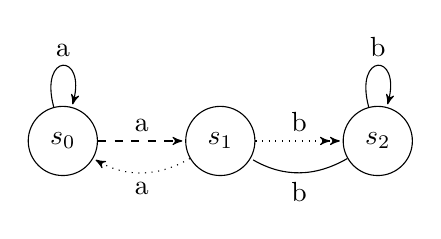
\begin{tikzpicture}[>=stealth',shorten >=1pt,auto,node distance=2cm]
  \node[state] 	       (s0)               {$s_0$};
  \node[state]         (s1) [right of=s0]  {$s_1$};
  \node[state]         (s2) [right of=s1] {$s_2$};
%  \node[state]         (s3) [right of=s2]  {$s_3$};
 % \node[state]         (s4) [under of=s0] {$s_4$};
  

  \path[->]          (s0)  edge [loop above] node {a} (s0);
  \path[->, dashed]  (s0)  edge              node {a} (s1);
  \path[->, dotted]  (s1) edge [bend left]  node {a} (s0);
  \path[->>, dotted] (s1) edge             node {b} (s2);
  \path              (s2) edge [loop above] node {b} (s2)
             edge [bend left]  node {b} (s1);
\end{tikzpicture}
\end{document}
